\documentclass[11pt]{article}

\usepackage{fullpage}
\usepackage{graphicx}
\graphicspath{ {./images/} }

\begin{document}

\title{ARM11 - Assembler, Emulator and Extension}
\author{Group 10}

\maketitle

\section{Introduction}
This report provides an analysis of our group's work on the ARM11 project, our extension and the way we managed the tasks.

\section{Group Organisation}
We began the work on the project by reading and understanding the specifications and summarizing all the information on a team management platform, Trello, which allowed us to make notes ans set tasks. Afterwards, we split the tasks and started work while continuously keeping track of our progress and setting new goals.  \\ \par \noindent
Since we were all beginners in C programming, we decided to work together in the early stages of our project. We designed the ARM data structure, followed by the implementation of the memory and the registers, the three stage pipeline, interpreting the structure of instructions and reading from files. \\ \par \noindent
After implementing the core program and getting more familiar with C and with each other’s working behaviour, we decided each of us would program one of the four functions (Data Processing, Multiply, Single Data Transfer and Branch). Because some required more work than others (for example, the Multiply instruction was simpler), we tried to even out by pair coding when one was finished or taking up some parts that were necessary in the other person's code (for example, the computation of the Operand as an immediate value or as a register within Single Data Transfer, instead of Data Processing). \\ \par \noindent
To improve the readability and correctness of our code, we proof-read each other's code, added significant comments and found new ways to implement functions more efficiently. This was the case especially when debugging the code, which was done by the whole team as it entails a high level of attention to detail and different perspectives and ideas are needed. \\ \par \noindent
Pair coding has proven to be very effective, each of us coming up with new ways of writing the code in a more efficient way, or even discovering potential bugs/ typos as the code was written (such as bit masks errors or unnecessary pointer dereferencing). It also helped us to get to know each other even better and feel like a real team, not working only independently and then merging our solutions, but actually contributing to the whole project and learning from each other. \\ \par \noindent
Independent coding was also useful for developing our C knowledge. We all became aware of our personal C programming skill and, at the same time, it was also beneficial to understand how tasks should be distributed in a team. It made us fully aware of the attributions of a group member, each person having the same responsibilities and importance.
\\ \par \noindent
Since we found that it was very efficient, we decided to keep the same work style for the assembler: We all implemented the basic skeleton of the 2 passes, and then we split up the work by having each one of us do one separate type of function. When one of us was done with their function, the person would pair code with one of the other teammates.

\section{Implementation Strategies - Emulator}

We decided to structure the emulator by creating an ARM data structure, which contains the 17 registers as an array of 32-bit integers and the memory as an array of 64KB / 32 bit rows, making it 32-bit-addressable (since the instructions are 32-bit wide). It also contains the three-stage pipeline instructions: the fetched instruction, the decoded instruction and the currently executed one. \\ \par \noindent
What we may find challenging for the next part is the symbol table, because it is supposed to be an abstract data type that we have not yet encountered in C, which we will try to solve by reading tutorials and the notes of the following weeks of our C Programming course. Furthermore, the only parts of the Emulator that we think are reusable for the Assembler are the global variables (masks, registers indices) and the way we read the file, most of the new instructions being different from what we have programmed so far. \\


\section{Implementation Strategies - Assembler}
We implemented our assembler such that it goes through 2 passes. \\\par\noindent
In the first pass the assembler goes through every line of the input file, ignoring blank lines, and keeps track of the current address. If the line ends with the character ‘:’, it will store the label along with the address in the SymbolTable linked list.
It will also store the address of the last instruction as a global variable.\\\par\noindent
In the second pass the assembler goes through every line of the input file again (ignoring blank lines and labels) for each command it will then separate the mnemonic. It will then compare it with the values in the mnemonics array, it will call the function mnemonicFunc that will return a function pointer to one of the 5 functions that is required to process the command. Each command with take a number representing the type of command and also a char* holding the rest of the sting and will return a uint32\_t command that will then be printed to the output file.\\ \par \noindent
The assembler includes 2 linked lists which are defined in global.c, which also contains our global variables. \\ \par\noindent
The first one is called SymbolTable, and it stores the labels found during the first pass, along with their addresses. Its functions are addLabel, getAddress, initSymbolTable, and clearSymbolTable.
\begin{itemize}
\item addLabel(label, address) assigns the label and the address to end of the list, which is an empty node, and then creates a new empty node as the end of the list.
\item getAddress(label) assigns the label and the address to end of the list, which is an empty node, and then creates a new empty node as the end of the list.
\item initSymbolTable and clearSymblaetable are used to initialize and free the Symbol Table.
\end{itemize}
The second one is called LDRTable, and it stores the data found in the LDR command that will be printed at the end of the instruction list.
\begin{itemize}
\item addData(data) assigns the data to end of the list, which is an empty node, and then creates a new empty node as the end of the list.
\item getData() returns the data at the head of the list and sets the head to head->next while freeing the old head.
\item initSymbolTable and clearSymbletable are used to initialize and free the LDR Table.
\end{itemize}
As mentioned above, there were 5 types of functions that had to be dealt with. These are:
\begin{itemize}
\item Branch Instructions, implemented in Branch.c
\item Data Processing Instructions , implemented in Data\_Processing.c
\item Single Data Transfer Instructions, implemented in Single\_Data\_Transfer.c
\item Multiply Instructions, implemented in Multiply.c
\item Special Instructions, implemented in Special.c

\end{itemize}

\section{Extension - "Pi-DJ"}
\subsection{Overview}
Our extension takes a premade template similar to a Synthesia snapshot that will have 50 lines, each with an option of 3 octaves of notes to be played at each time period. By editing the template and passing it as an argument to the program, the program will start from the top line and play each chord of notes. \\
The purpose of the app is to have fun with music and create a simple template for anyone to create tunes. This could be useful for music lessons aimed at children, helping them gain an understanding of musical notes.\\
We will work on making the project more user friendly by next week, as our current version works only on premade templates.
\subsection{Implementation Details}
Our program reads the pixel colour data of a png file which follows a predefined template, shown above in Figure 1. \\
\begin{figure}
\centering
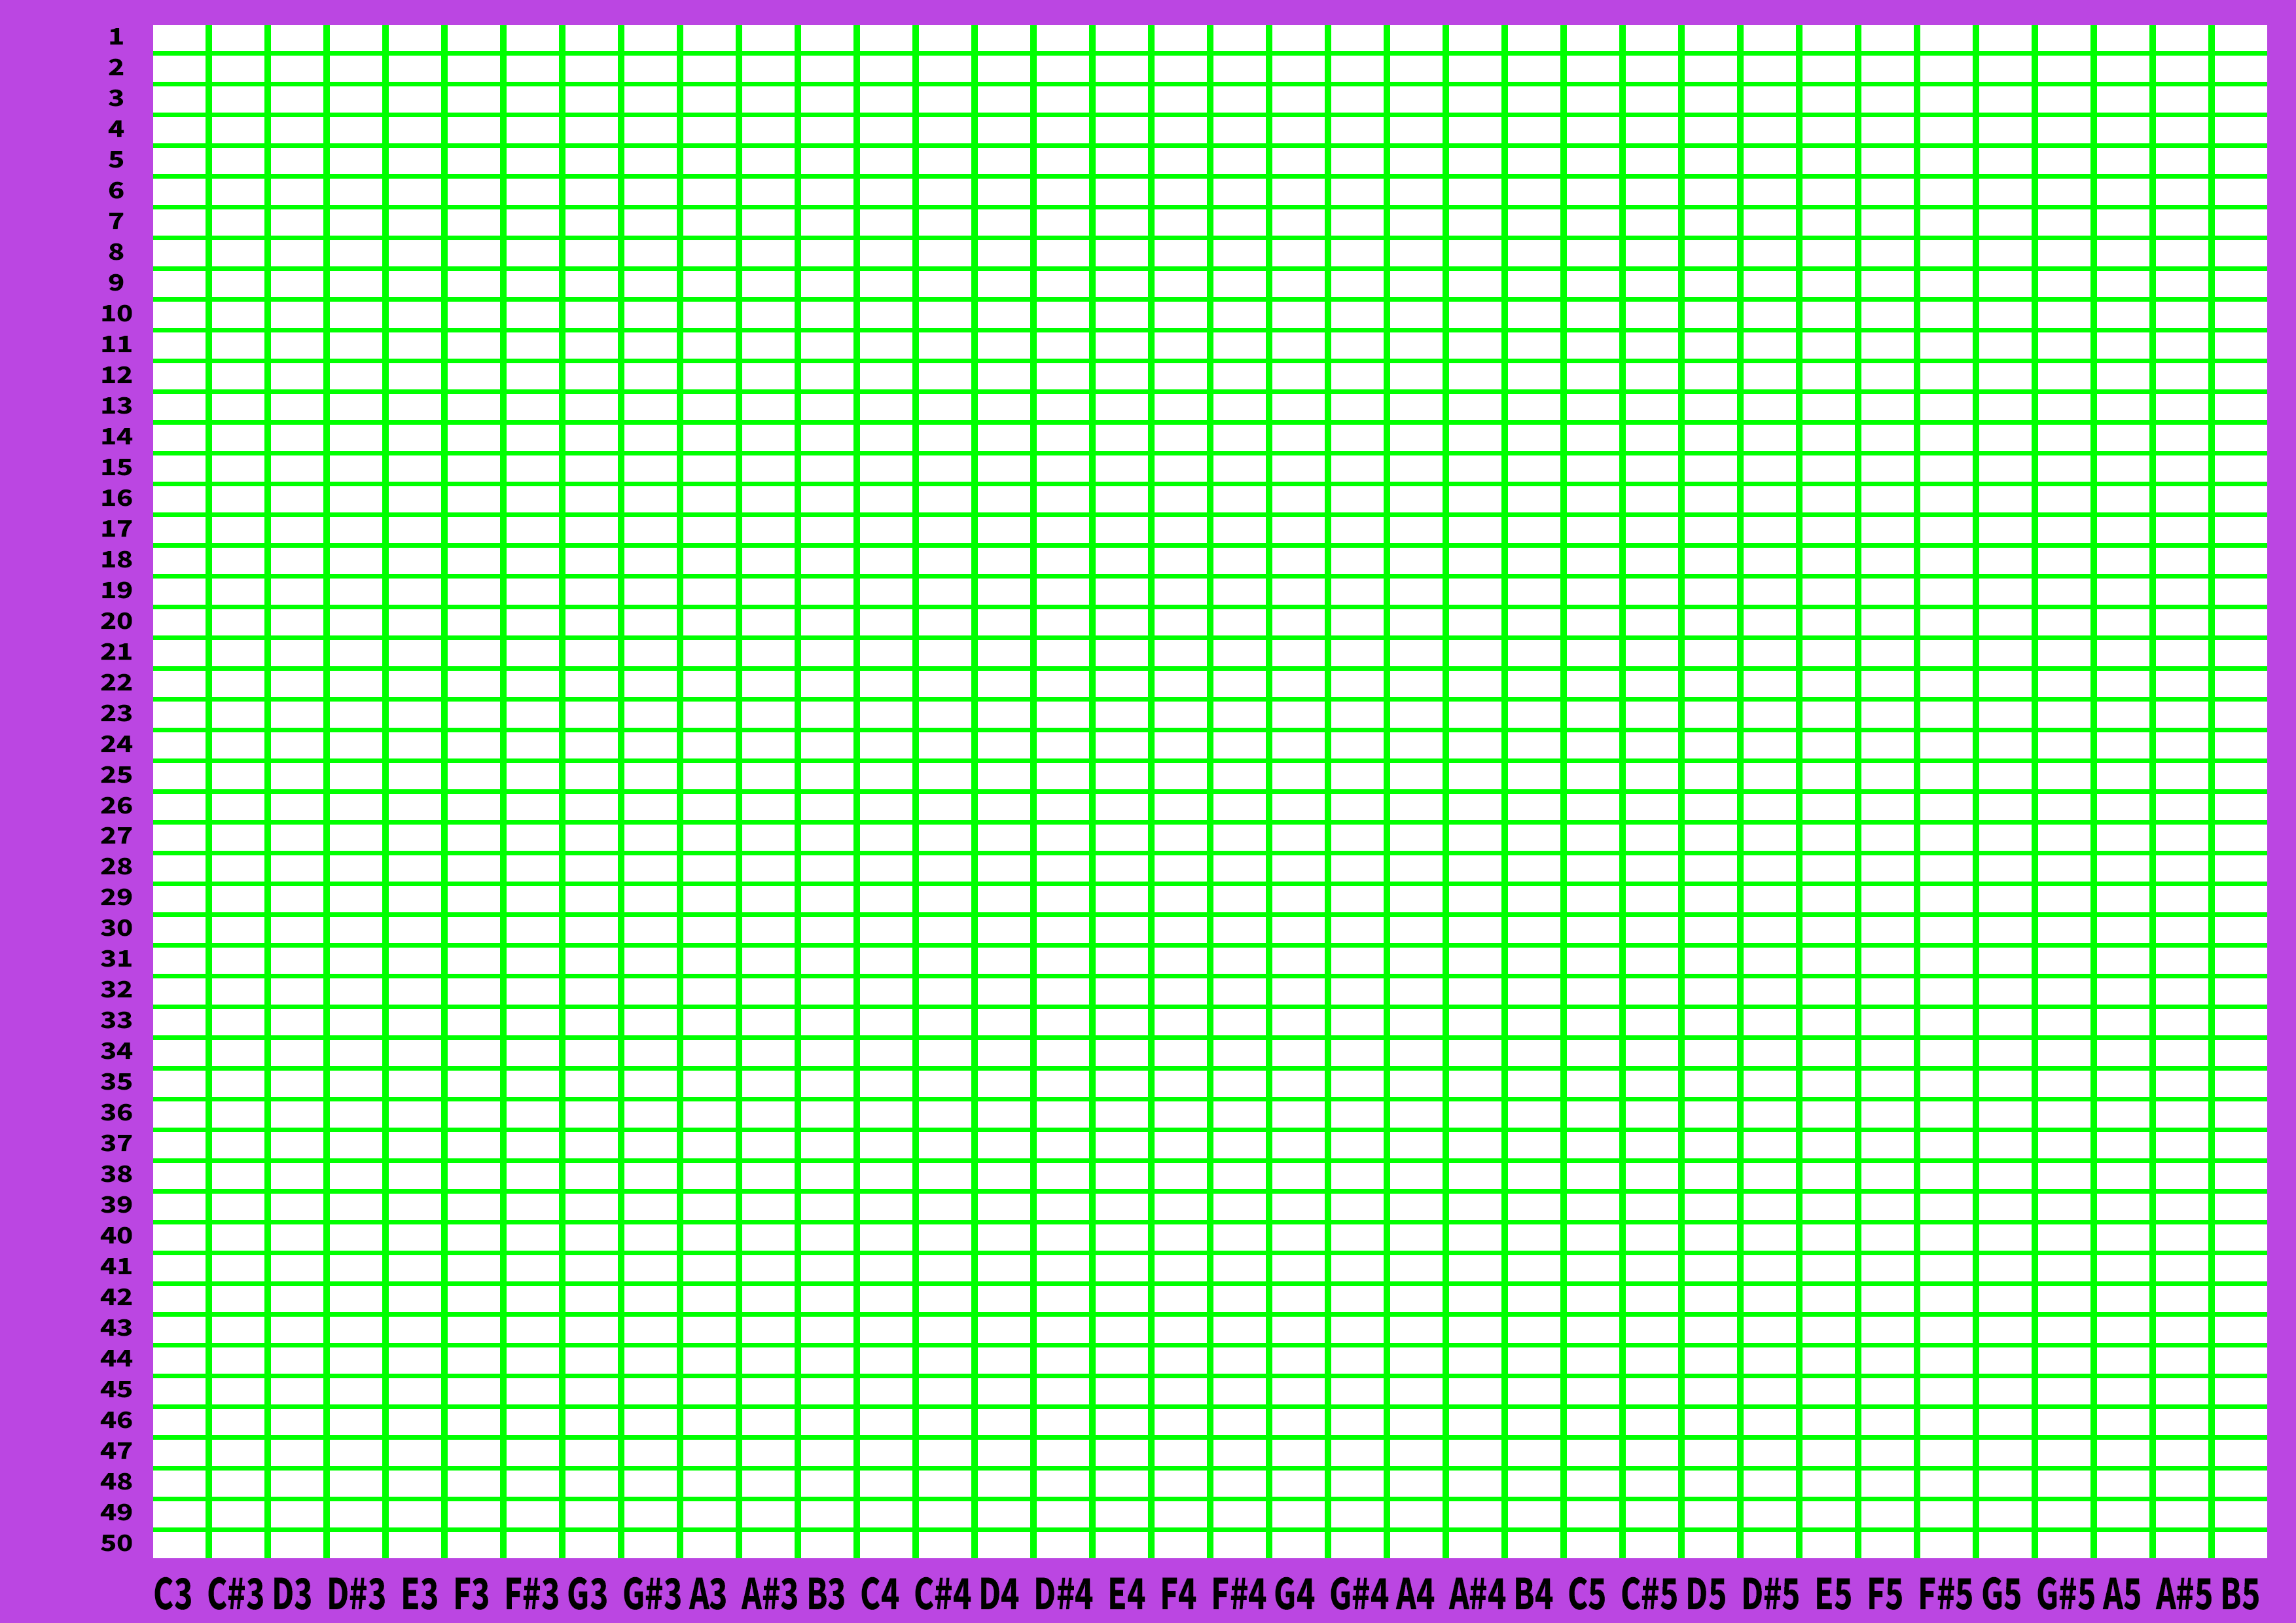
\includegraphics[width=120mm]{empty}\\
\title Figure 1
\end{figure}
Then we processing from top to bottom, each line of the grid representing one time period. Processing one line of the grid consists of parsing it from left to right, until an orange tile is found, which would represents one single note that would be played for that time period. Our implementation allows a total of 6 notes per row, because it's not usual for a chord to have more than 6 different sounds. \\
In order to generate sounds we used the SoX audio editing software. A SoX command is generated and played by each processed row. \\
If the program encounters an empty row, it signals a pause of 0.3 seconds. This is used as a way to moderate time periods. \\ \par
The challenges we encountered while developing our extension were:
\begin{itemize}
\item Understanding how to include libraries when compiling code. In our case we had to use -lpng.
\item Searching and understanding a library to read pixel colors of a picture.
\item Understand using the Sox audio manipulation language.
\item String concatenation and allocating memory for char*.
\end{itemize}

\subsection{Testing}
We created two template png files for “Twinkle Twinkle Little Star”. One with single notes and another with chords (Figure 2) to test the functionality of the program.
\begin{figure}
\centering
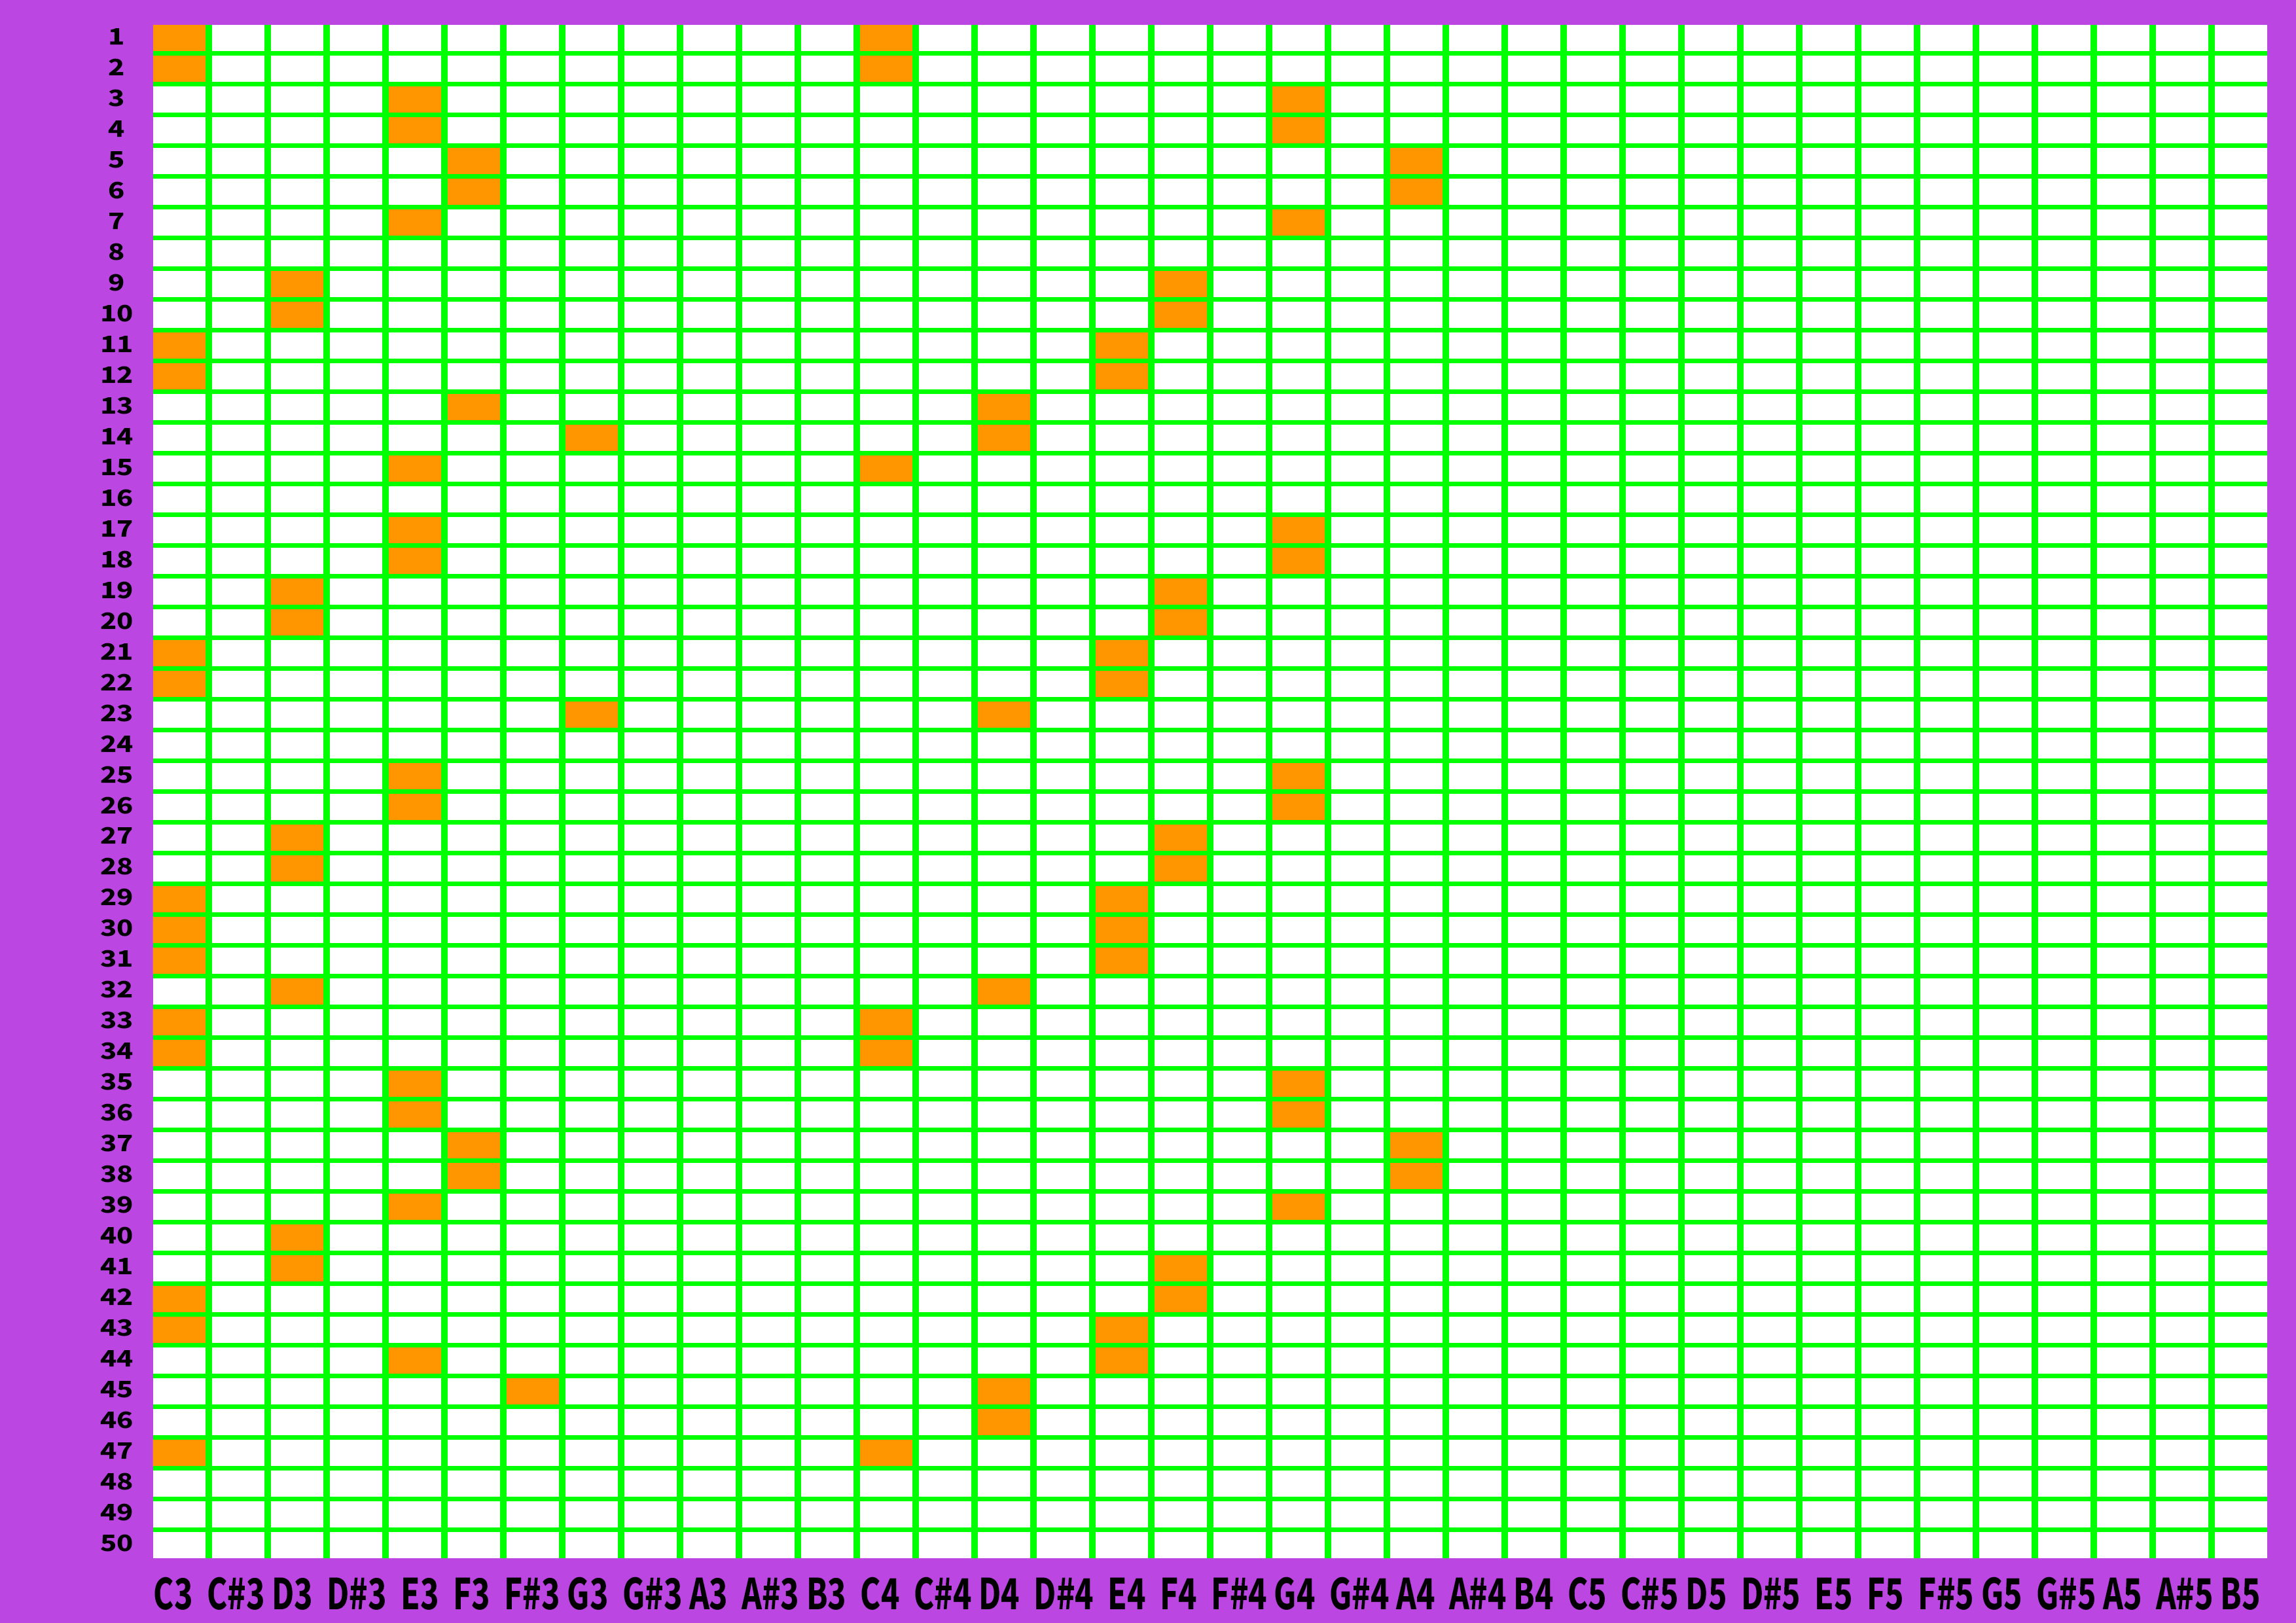
\includegraphics[width=120mm]{twinkle_chords}\\
\title Figure 2
\end{figure}

\section{Team's reflections}

Here are some reflections on the project and how our team functioned together. \par \noindent
\subsection{Team Reflection}
It was a very good idea to use a project management app because it enabled us to work more efficiently. We all learned how to properly use git together, which was very important for all of us. Some people in the team are better at programming, while the others are better at problem solving, so in the end this made our team very well rounded.
\subsection{Iulia}
I found that our team worked very well together, and we didn't really have any conflicts. This was the first time I was in charge of a team, and it helped me learn how to allocate tasks so that work gets done efficiently. I also really enjoyed our extension since we got to do something we all enjoyed.

\subsection{George}
Completing my assigned tasks helped me further my knowledge in C programming. Creating the make file taught me a very important skill and working with linked lists helped me understand structs in C very well. I had no trouble working with the team, as we had very similar work ethics.

\subsection{Maria}
Since we were already friends, it was easy for us to work together. I very much enjoyed the extension because it allowed us to think creatively and do something music-related, which we all love. Given that this was our first programming group project I’m really happy with the way we managed it.
\subsection{Miruna}



\end{document}
